\documentclass[tikz,border=8pt]{standalone}
\usepackage{amsmath,amssymb}
\usepackage{tikz}
\usetikzlibrary{arrows.meta,calc}

\begin{document}
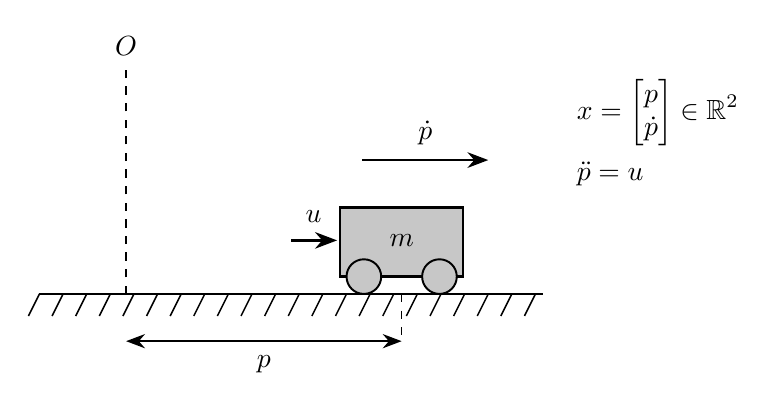
\begin{tikzpicture}[
  >=Stealth,
  font=\normalsize
]
  % ground
  \draw[line width=0.95pt] (-3.4,0) -- (3.0,0);
  \foreach \x in {-3.4,-3.1,...,2.9}
    \draw[line width=0.55pt] (\x,0) -- ++(-0.14,-0.28);

  % origin
  \draw[dashed, line width=0.55pt] (-2.3,0) -- (-2.3,2.85);
  \node[anchor=south] at (-2.3,2.90) {$O$};

  % classic cart: axle on body bottom, wheels half below (centers at y = r)
  \filldraw[fill=black!22, draw=black, line width=0.9pt]
    (0.42,0.22) rectangle (1.98,1.10);
  \node at (1.2,0.68) {$m$};
  \filldraw[fill=black!22, draw=black, line width=0.7pt]
    (0.72,0.22) circle (0.22);
  \filldraw[fill=black!22, draw=black, line width=0.7pt]
    (1.68,0.22) circle (0.22);

  % position p
  \draw[<->, line width=0.85pt] (-2.3,-0.60) -- (1.2,-0.60);
  \node[anchor=north] at (-0.55,-0.66) {$p$};
  \draw[dashed, line width=0.45pt] (1.2,0) -- (1.2,-0.60);

  % input u
  \draw[->, line width=1.1pt] (-0.20,0.68) -- (0.38,0.68);
  \node[anchor=south] at (0.08,0.78) {$u$};

  % velocity
  \draw[->, line width=1.0pt] (0.70,1.70) -- (2.30,1.70);
  \node[anchor=south] at (1.50,1.77) {$\dot{p}$};

  % equations
  \node[anchor=north west, align=left] at (3.3,2.85) {%
    $\displaystyle x=\begin{bmatrix}p\\ \dot{p}\end{bmatrix}\in\mathbb{R}^{2}$\\[5pt]
    $\displaystyle \ddot{p}=u$%
  };
\end{tikzpicture}
\end{document}
